\documentclass[10pt, a4paper]{article}
\usepackage[spanish]{babel} % espanol.
%Lo pongo en english para que me compile :S.

\usepackage[utf8]{inputenc}
\usepackage{enumerate} % enumerados
\usepackage{graphicx}
\usepackage{longtable}
\usepackage{multicol}
\graphicspath{ {img/} }
\usepackage[paper=a4paper, left=1.5cm, right=1.5cm, bottom=1.5cm, top=3.5cm]{geometry}
\usepackage{indentfirst}
\usepackage{fancyhdr}
\usepackage{color}
\usepackage[colorlinks=true, linkcolor=black]{hyperref}
\usepackage{a4wide}
\usepackage{tikz}
\usepackage{epsf}
\usepackage{caratula}
\usepackage[]{algorithm2e}
\usepackage[]{algorithmic}
\begin{document}


\begin{figure}[ptb]

\includegraphics[scale=0.30]{logo.jpg}\hspace{6cm}

\includegraphics[scale=0.90]{logo_dc.jpg}
\end{figure}

%Datos de la caratula
\materia{Redes Neuronales}
\titulo{Trabajo pr\'actico 1}
\subtitulo{Parser}
\hspace{6cm}
\integrante{Negri, Franco}{893/13}{franconegri2004@hotmail.com}
\integrante{Rey, Martin Gaston Podavin}{483/12}{marto.rey2006@gmail.com}
\palabrasClave{TP}
  % Reconocimiento caras. PCA. Power Method. Deflation. Autovalores. Autovectores. Matriz
  % semi definida positiva.

\resumen{Entrenamiento de Redes Neuronales}

\parskip=5pt % 10pt es el tamaño de fuente

% Pongo en 0 la distancia extra entre ítemes.
\let\olditemize\itemize
\def\itemize{\olditemize\itemsep=0pt}

% Acomodo fancyhdr <- Creo que es el encabezado de pagina
\pagestyle{fancy}
\thispagestyle{fancy}
\addtolength{\headheight}{1pt}
%\lhead{Acosta, Negri}
%\rhead{1$^{do}$ Cuatrimestre 2016}
\cfoot{\thepage}
\renewcommand{\footrulewidth}{0.4pt}




%Pagina de titulo e indice
\thispagestyle{empty}

\maketitle



\tableofcontents
\pagebreak
\section{Introduccion}
En este trabajo practico buscamos modelar el juego de 4 en linea y jugadores que utilicen técnicas de q-learning. Además exploraremos distintas políticas de exploración para utilizar en un jugador y veremos que impacto tiene cada una de ellas en los resultados obtenidos. 

Para finalizar, realizaremos distintos experimentos con el objetivo de observar de manera empírica que sucede al variar parámetros tales como el coeficiente de aprendizaje, la inicialización de la matriz Q o entrenándolo contra otros tipos de jugadores.

Algo interesante para notar aquí es que, en este juego se contará con la participación de dos agentes que compiten entre ellos, por lo que deberá prestarse particular atención en como se modelará la etapa de recompensa del algoritmo.
\section{Desarrollo}
\section{Modelado}

\subsection{Modelado del juego}

La estructura de datos que utilizaremos para modelar este juego consistirá en una lista de listas: cada una de ellas representará una columna del tablero. En cada turno, se le entregará el estado actual del tablero al jugador y este elegirá una columna numerada del $0$ al $n$ (siendo $n$ el numero de columnas totales) y elegirá dónde colocar su ficha.

Luego de cada jugada, el juego chequeará si el jugador ganó o si ya no hay más movimientos posibles, terminando el juego e informando qué jugador ganó o si fue empate.

El pseudocódigo del juego será entonces el siguiente:

\begin{algorithm}[h!]
\begin{algorithmic}[1]\parskip=1mm
 \caption{jugar()}
 \STATE{While True}
 \STATE{\quad columna = player.move(tablero)}
 \STATE{\quad jugar\_ficha(columna, tablero)}
 \STATE{\quad if jugador\_gano(tablero)}
 \STATE{\quad\quad return player}
 \STATE{\quad if tablero\_lleno(tablero)}
 \STATE{\quad\quad return empate}
 \STATE{\quad player = otro\_jugador(player)}
\end{algorithmic}
\end{algorithm}

Como ya adelantamos en la introducción, es necesario definir en qué etapa del algoritmo se le asignará la recompensa al algoritmo de q-learning. Una opción bastante sencilla e intuitiva es la de asignar recompensas en el momento en que algún jugador gana la partida. Por ejemplo al ganar una partida, se le asigna una recompensa de $1$ al ganador y una recompensa de $-1$ a su adversario. Siguiendo con el lineamiento anterior, también sería posible asignarles recompensas en el momento en que se empata, por ejemplo, asignándoles a ambos jugadores una recompensa de $0.5$.

En caso de que no se haya llegado a un estado final, una posible propuesta es asignar una recompensa por ejemplo de $0$.

El pseudocódigo entonces, pasaría a verse de la siguiente manera:
\pagebreak
\begin{algorithm}[h!]
\begin{algorithmic}[1]\parskip=1mm
 \caption{jugar()}
 \STATE{While True}
 \STATE{\quad columna = player.move(tablero)}
 \STATE{\quad jugar\_ficha(columna, tablero)}
 \STATE{\quad if jugador\_gano(tablero)}
 \STATE{\quad\quad player.recompensa(1, tablero)}
 \STATE{\quad\quad otro\_jugador(player).recompensa(-1, tablero)}
 \STATE{\quad\quad return player}
 \STATE{\quad if tablero\_lleno(tablero)}
 \STATE{\quad\quad player.recompensa(0.5, tablero)}
 \STATE{\quad\quad otro\_jugador(player).recompensa(0.5, tablero)}
 \STATE{\quad\quad return empate}
 \STATE{\quad otro\_jugador(player).recompensa(0, tablero)}
 \STATE{\quad player = otro\_jugador(player)}
\end{algorithmic}
\end{algorithm}

Utilizando este modelo, en el siguiente apartado pensaremos cómo modelar un jugador que utilice esta estructura para implementar un algoritmo de q-learning.

\subsection{Modelado de jugadores}

Un jugador estará compuesto por dos métodos básicos, uno que llamaremos $move()$ que, dado un estado del tablero devuelve una acción valida (tirar una ficha en la primera columna, en la segunda, etc) y una función $reward()$ que nos dirá en qué estado quedó el juego luego de movernos y de que el oponente moviera, y una recompensa que utilizaremos para actualizar la matriz $Q$ en caso de que el jugador lo requiera.

En particular, para la clase Jugador que implemente q-learning, el algoritmo para decidir qué acción realizar vendrá dado de la siguiente manera:

\begin{algorithm}[h!]
\begin{algorithmic}[1]\parskip=1mm
 \caption{move(tablero)}
 \STATE{acciones\_validas = elegir\_acciones\_validas(tablero)}
 \STATE{Para cada acción en acciones\_validas}
 \STATE{\quad obtener q para accion}
 \STATE{\quad guardarlo en lista de qs\_validos}
 \STATE{accion\_elegida = elegir\_acción(acciones\_validas,qs\_validos)}
 \STATE{retornar accion\_elegida}
\end{algorithmic}
\end{algorithm}

Y la función learn, que básicamente consiste en adaptar la función de aprendizaje vista en la teórica:

\begin{algorithm}[h!]
\begin{algorithmic}[1]\parskip=1mm
 \caption{learn(tablero,recomensa)}
 \STATE{prev\_q = getQ(estado\_previo, accion\_elegida)}
 \STATE{maxqnew = tomar maximo q de tomar una acción en el tablero resultante}
 \STATE{q[(estado\_previo, accion\_elegida)] = prev + $\alpha$ * ((reward + $\gamma$*maxqnew) - prev)}
\end{algorithmic}
\end{algorithm}

Aquí quedan por definir varios parámetros, entre ellos $\alpha$, $\gamma$ y los valores iniciales para la matriz $Q$. En primera instancia decidimos tomar valores que consideramos apropiados de acuerdo a resultados empíricos que realizamos a priori y que consideramos razonables. Tomaremos $\alpha=0.4 $, $\gamma=0.9$ y todas los valores de Q iniciarán con $1$ con el objetivo de alentar la exploración.

Además de la metodología descripta anteriormente se nos ocurrieron otras heurísticas interesantes, que por falta de tiempo o por ser simplemente malas, no indagamos en profundidad. Una de ellas consistía en utilizar el estado siguiente (aquel perteneciente al jugador rival para determinar el mejor movimiento). La idea básica era, para cada acción, tomo su q, realizo una transición por ese estado, invierto el tablero (las fichas rojas pasan a ser azules y las azules pasan a ser rojas) y le resto el mejor q de este otro estado. Pensamos que de esta manera estaríamos agregando información útil sobre potenciales buenas jugadas del contrincante a nuestra fase de decisión, pero en la práctica daba malos resultados.

Otra heurística interesante surgió de la siguiente idea: cuando pierdo, no solo sé que pierdo, sino que sé que el otro ganó y no solo eso, también sé \textit{cómo} ganó. En base a eso una idea muy interesante para explorar era, al momento de recibir una recompensa realizar $learn(invertir(tablero), -recompensa)$, donde $invertir$ funcionaría invirtiendo las fichas rojas por azules y viceversa. Si bien implementamos esto, dado que los resultados obtenidos no variaron significativamente y que nos encontrábamos al final de la etapa de experimentación, los siguientes apartados no reflejan ni tienen en cuenta esta posible mejora.

En la siguiente sección terminaremos de definir la función $elegir\_accion()$ basándonos en distintas heurísticas para resolver el problema del Multi-armed bandit.

\subsection{Estrategias de movimiento}

Aquí plantearemos distintas estrategias que utilizará nuestro jugador al momento de elegir: si decide explorar nuevos caminos o decide utilizar el mejor camino conocido hasta el momento.

La primera heurística que elegimos implementar es una estrategia greedy en donde el jugador tomará un camino random con probabilidad $\epsilon\%$ y en caso contrario utilice el mejor brazo conocido. Es claro que dependiendo de este valor $\epsilon\%$ nuestro algoritmo será mas propenso a explorar o a elegir el mejor camino posible.

La segunda estrategia es conocida como $\epsilon$-first: en este caso el jugador toma un camino random en las primeras $\epsilon$ iteraciones y luego toma el mejor camino conocido. Esperamos que en estas $\epsilon\%$ iteraciones el jugador explore una gran cantidad de estados posibles, tras los cuales podrá decidir con más confianza cuál es el mejor camino a elegir.

Como última heurística utilizaremos una estrategia Softmax: basada en una función probabilística, la estrategia Softmax se basa en darle probabilidades distintas a cada acción posible dependiendo de la recompensa esperada de cada una de ellas.

En particular la probabilidad de cada una de las acciones vendrá dada por:

$$P_t(a) = \frac{\exp(q_t(a)/\tau)}{\sum_{i=1}^n\exp(q_t(i)/\tau)}$$

Donde $q_t(a)$ es el valor del valor esperado siguiendo la acción $a$ y la variable $\tau$ se denomina ``parámetro de temperatura''. Para temperaturas cercanas a infinito, todas las acciones tienen aproximadamente la misma probabilidad de ser elegidas, mientras que para temperaturas bajas (cercanas a cero) la probabilidad de la acción de mayor recompensa tenderá a $1$.

En particular nuestra estrategia consistirá en comenzar con una temperatura alta para favorecer la exploración e ir gradualmente disminuyéndola para favorecer más a aquellas con mayor recompensa. Faltará definir de alguna manera cuál será el valor inicial de $\tau$ y de qué manera reduciremos su valor (algunas posibilidades son de manera lineal, logarítmica, etc). De esta manera esperamos que en situaciones donde todos los qs tengan valores similares, el jugador sea más propenso a explorar nuevos caminos mientras que en situaciones críticas (estando cerca de un estado ganador) elija el camino con mayor recompensa.

\subsection{Análisis: espacio de estados}

Según el modelo planteado para la resolución del problema, la matriz Q tendrá como columnas los diferentes estados en los que se puede encontrar el tablero y como filas, las acciones que se pueden realizar sobre ese determinado tablero. Dado que la cantidad de estados diferentes en los que se puede encontrar el tablero tiene complejidad PSPACE y que la cantidad la acciones es acotada (a lo sumo $m$), podemos determinar que la complejidad espacial de nuestro algoritmo está en PSPACE... \textit{not cool}.

Si bien esto hace que la complejidad de explorar cada una de las posibilidades sea extremadamente costosa, consideramos que para la mayoría de los casos no es necesario conocer todo el árbol sino los estados más generales.

%referencia http://www.tzi.de/~edelkamp/publications/conf/ki/EdelkampK08-1.pdf


\pagebreak
\section{Experimentación}

\subsection{Estrategias vs jugador random}

Como primera instancia en la etapa de experimentación, haremos competir a un jugador q-learner contra un jugador que elige entre los posibles movimientos con probabilidad uniforme (random). Utilizaremos las tres estrategias descriptas previamente para ver cómo se comporta cada una. 

La metodología utilizada para observar cómo evoluciona el algoritmo de q-learning será la de hacer jugar a ambos jugadores $10000$ veces, randomizando cual es el que comienza primero en cada iteración. Luego tomaremos estos resultados y cada $250$ juegos, graficaremos cuántas veces ganó el algoritmo q-learning. 

Para la estrategia greedy, tomando $\epsilon=0.1$ obtuvimos los siguientes resultados:

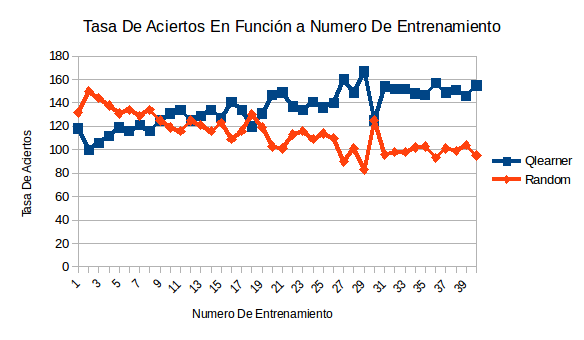
\includegraphics[scale=0.5]{testing/greedy.png}

Puede observarse, a medida que pasa el tiempo, cómo el jugador q-learner empieza a converger a una estrategia ganadora, obteniendo al final del experimento un $16\%$ más de aciertos que el jugador random.

Para la estrategia $\epsilon$-first tomando $\epsilon=10\%$, resultados fueron los siguientes:

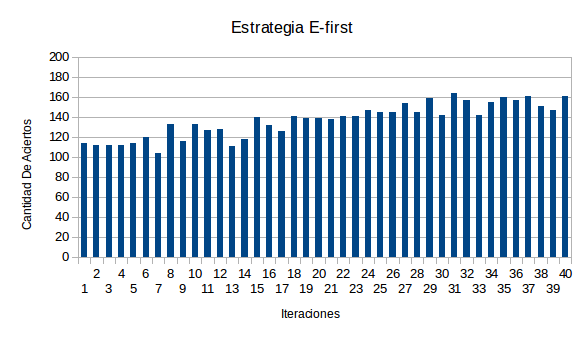
\includegraphics[scale=0.5]{testing/ef.png}

Puede verse cómo en el primer $10\%$ de las iteraciones el algoritmo gana la mitad de las veces y pierde la otra mitad, lo que era de esperarse para una política completamente random. Pasadas esta cantidad de iteraciones, puede verse un repentino crecimiento en la cantidad de partidas ganadas, llegando al final a casi un $32\%$ más de aciertos que su adversario.

Con la tercera política Soft-Max, decidimos utilizar una temperatura inicial igual a $1$ y una función de calor que desciende de manera logarítmica con cada iteración:

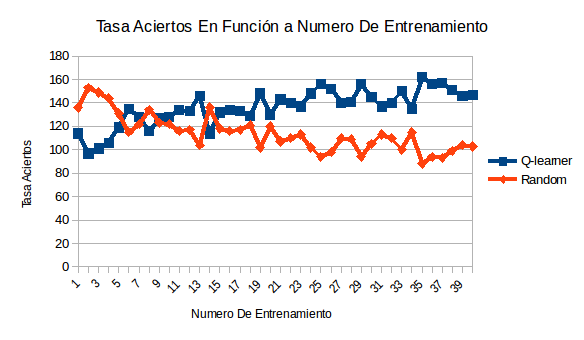
\includegraphics[scale=0.5]{testing/softmax.png}

Aquí al igual que en los algoritmos vemos un crecimiento en la tasa de aciertos a medida que se cumplen una mayor cantidad de iteraciones. Aun así esperábamos una mayor diferencia comparado con los otros dos algoritmos, siendo este el que utiliza más información de la matriz Q. Consideramos que posiblemente esto se debe a que los parámetros particulares de este método estuvieran mal ajustados, pero tras intentar con diferentes valores, no logramos obtener una mejora notable.

A modo de conclusión, podemos decir que la heurística que se divide en dos etapas, una puramente exploratoria y otra donde se utiliza esta información, resultó ser la mas efectiva. Seguramente esto suceda ya que en la fase exploratoria se llegan a explorar muchos caminos diferentes, los cuales en la etapa de ``explotación'' utilizaremos el mejor. En cambio en estrategias como greedy y Softmax, al tener siempre una probabilidad considerable de elegir el mejor camino, estemos sesgando al algoritmo para intentar llegar siempre a la misma solución o a soluciones similares que tal vez no sean las óptimas para ese juego en particular.

\subsection{Performance de dos q-learners compitiendo}

En esta sección analizaremos el comportamiento de dos jugadores q-learners (ambos utilizando una estrategia greedy) compitiendo entre sí y aprendiendo al mismo tiempo. Lo que esperamos observar es que tras un período donde ambos jugadores obtienen una tasa de aciertos cercana al $50 \%$, esta tasa empiece a converger a un numero más bajo a medida que ambos converjan a una misma estrategia ganadora y empaten en más oportunidades. Los resultados obtenidos fueron los siguientes:

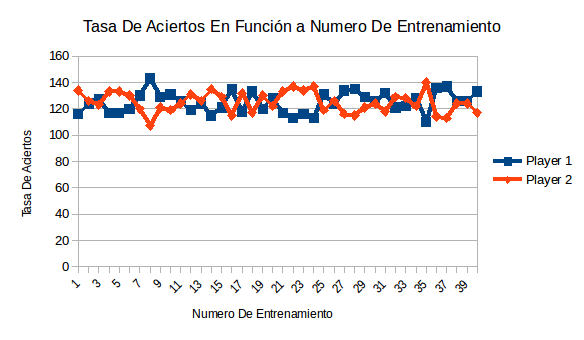
\includegraphics[scale=0.5]{testing/qvsq.png}

Se realizó la misma experimentación con las otras dos estrategias, obteniéndose resultados similares en ambos casos. Esto no aproxima a los valores esperados, una hipótesis posible es que el jugador que juega primero tenga más ventaja que el que juega segundo y por lo tanto, al estar randomizado el orden en que empiezan, la mitad de las veces gane uno y la otra mitad gane el otro. Para testear esto modificamos el programa para que el jugador 1 siempre comience primero y el jugador 2 siempre comience segundo:

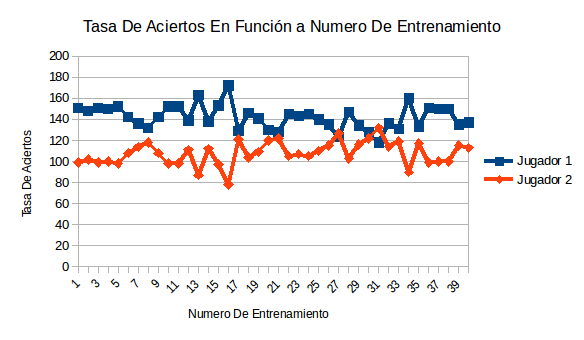
\includegraphics[scale=0.5]{testing/qvsq2.png}

La hipótesis parece confirmarse dado que el primer jugador obtiene un $20 \%$ más de partidas ganadas que el segundo.

\subsection{Performance al cambiar la inicialización de Q}

En el siguiente experimento buscamos ver qué sucede al variar entre distintos valores iniciales la matriz de Q. Para ello utilizaremos un jugador random y un jugador q-learning con estrategia greedy y variaremos Q. Como primer experimento cambiaremos el valor inicial de $1$ a $0$. De esta manera, esperamos desalentar la fase de exploración del algoritmo y que se guíe en mayor grado por el camino óptimo encontrado hasta el momento. Los resultados fueron:

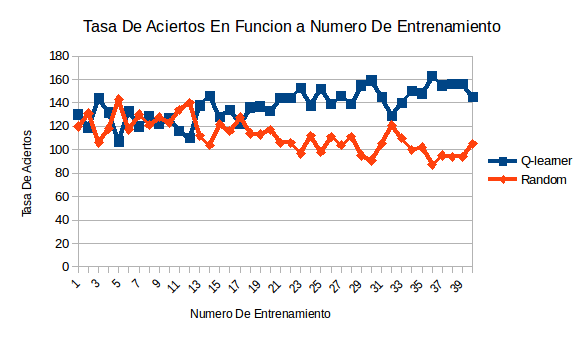
\includegraphics[scale=0.5]{testing/variarq.png}

Los resultados no parecen ser muy afectados por este cambio. Otra alternativa intermedia que ideamos podría ser inicializar los valores de Q con valores aleatorios en un rango definido, randomizando entonces un poco más cuáles caminos son explorados y cuáles no. Esperamos que de esa manera se exploren caminos que tal vez en otras circunstancias no fueran explorados y que esto mejore la performance a largo plazo. En el siguiente experimento la matriz Q está inicializada con distribución uniforme en el rango $[-1,1]$:

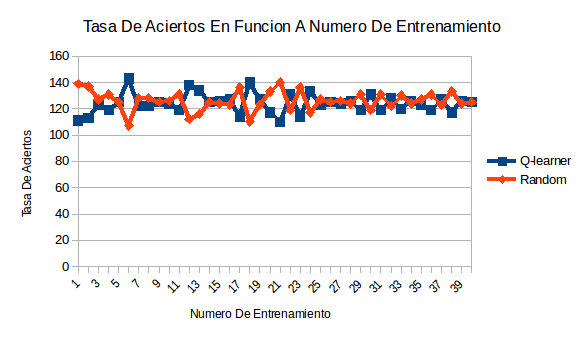
\includegraphics[scale=0.5]{testing/variarq2.png}

Como puede verse este tipo de exploración arrojó resultados muy malos, inducidos posiblemente por la dificultad de elegir un buen camino habiendo una tasa tan alta de ruido en el Q inicial.
\section{Concluciones}
No pudimos terminar el trabajo práctico como quisimos por malos manejos con los tiempos que nos dieron y porque no pudimos combinarlos de la mejor forma entre los integrantes del grupo (a causa de parciales, trabajo, entre otras cosas). Sin embargo, dejamos escrito aquí qué es lo que nos parece que falta y hubiera aportado mucho a este trabajo:

Elegimos usar Random Forest ya que en el siguiente paper [1] obtienen buenos valores de Accuracy, Precision y Recall. Tambien encontramos varias comparaciones entre naive bayes y random forest. En el siguiente paper [2] hay una comparacion entre que tipo de naive bayes mejoraba la clasificacion de spam. Estos eran Bernoulli multi variada NB y Multinomial NB. Concluyen que el que mejor clasificaba era Multinomial NB pero nosotros no logramos adaptar los hiperparametros para obtener resultados que se asemejen debido a la falta de tiempo. Llegamos a separar a partir de los datos que nos brindaron, un subconjunto que sea una caja negra para luego de configurar todos los hiperparametros de los clasificadores, usarlos y quedarnos con el que mejor accuracy brinde. Nos hubiera gustado calcular las matrices de confusion y ROC (como asi tambien la accuracy, precicion y recall) sobre estos resultados obtenidos clasificando dicho subconjunto.


[1] http://www.irdindia.in/journal_ijacect/pdf/vol2_iss4/1.pdf
[2] http://www.aueb.gr/users/ion/docs/ceas2006_paper.pdf

\end{document}

